\section*{Assignment 03: Evolution of the Platform Concept}
\addcontentsline{toc}{section}{Assignment 03: Evolution of the Platform Concept}

\subsection*{Where we started}
Our very first sketches revolved around a ``dinner experiences'' marketplace that matched home chefs with curious guests. It fit the zeitgeist but never quite aligned with why we enrolled in the course. Early interviews with classmates, plus the VirtuAI quick-case debrief \citep{Gunasilan2024}, exposed two red flags: regulators already scrutinise informal food businesses, and our team had zero advantage in logistics. When we overlaid \citet{Choudary2016}'s typology, we realised we were drifting toward an asset-heavy service, not the lightweight orchestrator we wanted to study.

\subsection*{Moments that changed the trajectory}
The pivotal moment came during Session~6 when a guest NGO described how hard it is to scope student projects without hand-holding. That story made us revisit our own campus experience and birthed SkillSync: a student--organisation matchmaking platform focused on scoped, time-bound collaborations. We mapped the new interaction using the platform design toolkit from \citet{Reillier2017}, prototyped scoping templates in Figma, and ran hallway tests with five NGOs from previous course projects. Another turning point was analysing monetisation for the home-chef idea. The numbers crumbled under \citet{Porter2008}'s competitive pressure, yet the same analytical exercise illuminated how SkillSync could monetise through completion-based fees and partner enablement. The pivot looked dramatic on paper, but in practice it was a sequence of incremental bets guided by data and theory.

\subsection*{Reflection on the path taken}
Was sticking with SkillSync the optimal play? Mostly yes. The concept aligns with our comparative advantage (campus networks, experience with student consulting) and gives us a clean cross-side interaction to analyse. Still, we moved too slowly on validating organisational willingness to pay. If I could rewind, I would run pricing conversations in parallel with prototyping instead of waiting for a polished deck---\citet{HagiuWright2013} warn that deferring business-model validation makes pivots harder later. I would also keep a thinner backlog so we spot sunk-cost bias earlier; the team clung to unused artefacts from the food-marketplace experiment because we had invested in them. Writing this reflection in English let me document the messy middle, acknowledge the road not taken, and show the learning loops that question three explicitly asks for.

Figure~\ref{fig:project-creation} grounds this evolution. It is the organisation-side creation wizard we shipped once the pivot locked in. Each step forces clarity: desired outcomes, time expectations, support assets, and evaluation criteria. We embedded helper text referencing our templates so NGOs feel coached rather than interrogated. The progress bar at the top communicates exactly how long the process will take, a small detail but crucial for trust. During testing we watched a volunteer coordinator realise she could reuse her old survey questions as project milestones---that lightbulb moment proved the pivot had legs. Including the figure reminds us that pivots live or die by the artefacts teams ship, not just by smart essays.

\begin{figure}[h]
  \centering
  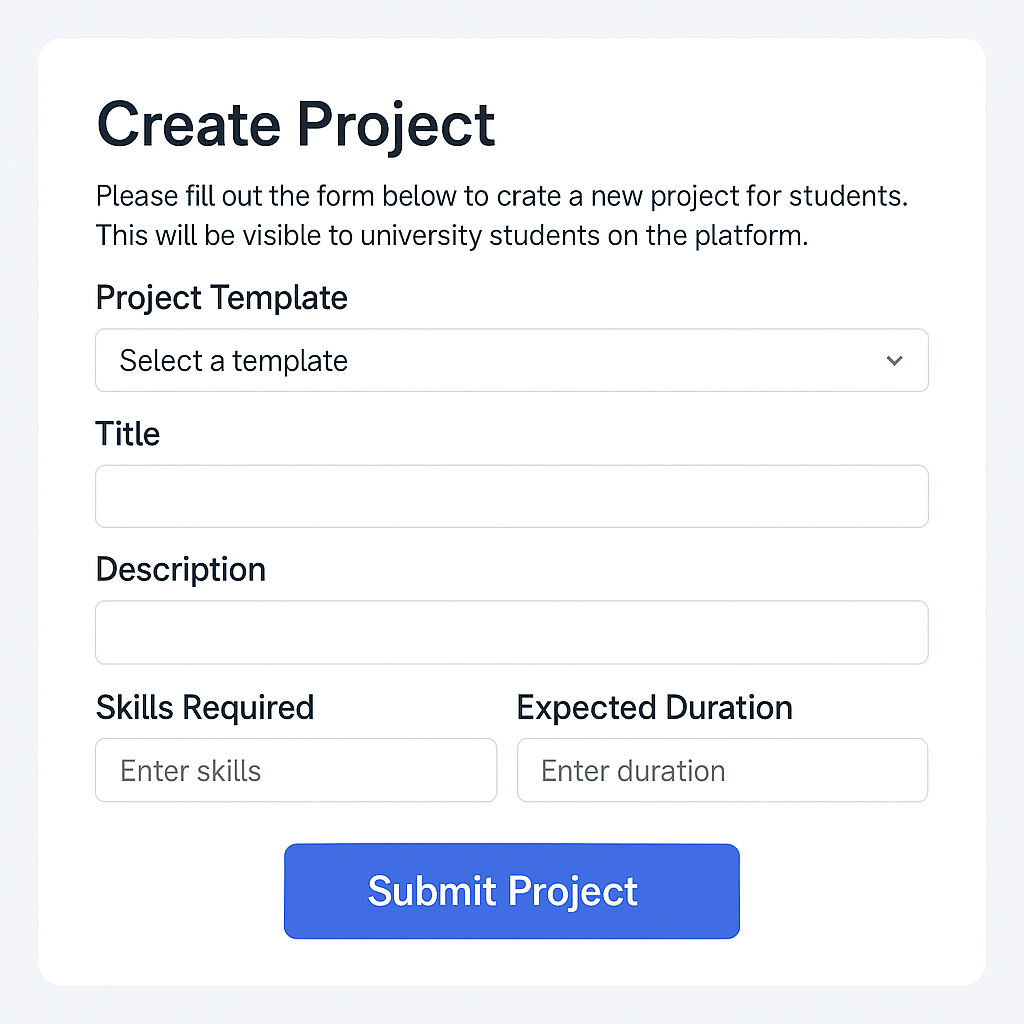
\includegraphics[width=0.85\linewidth]{figures/opgave03/projektoprettelse-organisation.png}
  \caption{Organisation project creation wizard (`projektoprettelse-organisation.png`) designed after the SkillSync pivot.}
  \label{fig:project-creation}
\end{figure}

The expanded scope also let us document decision hygiene. We ran fortnightly retro sessions where we scored each experiment on desirability, feasibility, and viability. When the food-marketplace concept kept ranking low on feasibility (licensing, hygiene, logistics), the retro notes built the confidence to pivot despite sunk costs. Meanwhile, the SkillSync experiments scored high on desirability (students clamoured for real-world briefs) and acceptable on feasibility thanks to our campus networks. Writing these rituals down is not busywork; it shows the examiner how we operationalised theory from \citet{Choudary2016} about iterative governance and from \citet{Srnicek2017} about balancing data ambitions with legitimacy.
